%!TEX program = <xelatex>
\documentclass{book}
\usepackage{mystyle}
\begin{document}

%!TEX root = <parallelTemperingMaster.tex>
%%%%%%%%%%%%%%%%%%%%%%%%%%%%%%%%%%%%%%%%%%%%%%%%%%%%%%%%%%%%%%%%%%%%%%%%%%%%%%%%%%%%%%%%%%%%%%%
\chapter{ Implementation }\label{Implementation}

In this chapter we will present the implementation of the \PTalgo, as described in \todo{Add Chapter on Theory}

The analysis of the algorithm in all its complexity called for the development
of a more structurised template for carrying out numerical computations. The
\PTalgo, being an extension to the \MHalgo, does naturally share many similarities its structure. Both algorithms can have very
abstract formulations and can be carried out theoretically on any countably-
generated measurable space. Practical considerations would never go that far.
However, one cannot, in principle, discard the use of Stochastic Simulations in solving many real-life modelling problems such as, for instance, the Bayesian model selection, or Ising-type modelling of crystallic structures. The mulitude of potential applications calls for a reasonably flexible implemention of the \PTalgo. To overcome these problems, the object-oriented paradigm was used in this work, so that the \sspace\, and the \algo\, were two separate entities. 

Having realised the need for modularity, it seemed natural to take the whole idea one step further and develop a general template for Metropolis-Hastings-like simulations, going way beyond the idea of a task-specific computer programme. For there are other potential developments of the \MHalgo\, that are being used, all baring strong similarities in stuctures of these algorithms. Our template's goal was therefore to provide basic building blocks used for simulations, leaving the practitioners concentrate on the analysis. The template is codenamed \ssimul \, and that shall be the \RR\, package name when shipped.


\RR\, offers several implemented meta-structures that enable basic object oriented programming techniques. Among these there are the \textbf{S3} classes, \textbf{S4} classes, and the most recent Reference Classes. The implementation the template, was carried out using Reference Classes. This choice was dictated by several reasons. First, only \textbf{S4} classes and Reference Classes offer the possibility of basic type verification\footnote{Still far from the \Cpp\, standards though.}. This assured that no serious errors were introduced in the implementation phase and that users cannot provide absurd input for the algorithm. Moreover, Reference Classes are claimed to be the only implementation of objects in \RR\, that use passing arguments by reference, and a priori could saved some time in the calculations on unnecessary object copying\footnote{No serious differences in execution time were actually spoted when comparing both the functionally programmed prototype with the object-oriented final version, however.}. Finally, Reference Classes are considered to be highly compatible with \Cpp\, precompiled programmes being called from \RR. This is a clear advantage, as the future shipments of \ssimul\, are planned to be implemented in \Cpp, so that users can simulate faster that the whole programme was more memory efficient.   

\section{Division into objects}

To assure real modularity of our template, more divisions were proposed than only the one mentioned at the beginning of this chapter. The overall structure is represented in Figure \ref{objectStructure}.

We already mentioned the separation of the \algo\, from the \sspace. It is useful to think of the \algo\, as of a decision-maker. Its role is restricted to making decisions on acceptance or rejections of the proposals generated by the \sspace\, and then on giving orders to the \sspace\, to perform subsequent actions. The information on which the \algo\, bases its decisions depends on the points from the \sspace\, only indirectly, via the evaluations of densities\footnote{In the discrete case -- probability functions} at the proposal points \todo{Mathy this by adding equations}.

 A third candidate for an entity thus appears - namely an object whose methods would serve to measure some characteristic of the \sspace\, sample points for the use in the decision-making of the \algo. We called this entity the \measure. 

The very idea behind the \measure\, entity is that it should serve as a container for user-defined probability function or a density together with every additional data-structure required for its evaluation. Moreover, in case the user was interested in testing the \PTalgo's potential against some analytically tractable toy-example, or in case this example was easy to simulate using a simpler or potentially more efficient technique than \mcmc, the \measure\,
 entity would be the place to store any additional method of carrying out calculations regarding this particular distribution. For example, in our simulations (confront Chapter \todo{simulationsAndResults}) we could  additionally provide efficient methods for quantile simulations and evaluates of the real distribuant. Implementations of these functions were collected as methods of the appropriately named instatiation of the \measure\, structure.  



\begin{figure}
	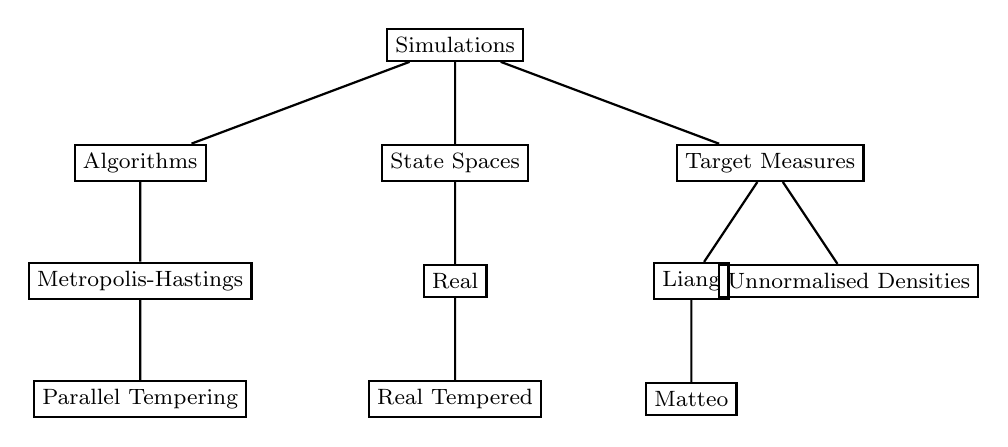
\begin{tikzpicture}
		[-,thick,%
		  every node/.style={shape=rectangle,inner sep=3pt,draw,thick}]
		\footnotesize
		\node {Simulations}
		  [sibling distance=4cm]
		  child {node {Algorithms}
		  	child {node {Metropolis-Hastings}
		  		child {node {Parallel Tempering}	
		  		}
		  	}	
		  }
		  child {node {State Spaces}
		    child {node {Real}
		    	child {node {Real Tempered}
		    	}
		    }
		  }
		  child {node {Target Measures}
		    [sibling distance=2cm]
		    child {node {Liang}
		    	child {node {Matteo}}
		    }
		    child {node {Unnormalised Densities}}
		  };
	\end{tikzpicture}
	\caption{Current operational entity-relations diagram.}\label{objectStructure}
\end{figure}

The reason for separating the \measure\, from the \sspace\, is again dictated by the modularity requirement. Totally different models can be modelled on the same \sspace\,, the only difference being the way the probability is assigned. It is therefore natural to define an entity whose task will be to serve as a warehouse for sample points, together with efficient methods or reading them, and in the end -- presenting the results to the user. These things, to some extent, can be done for any probability measure defined by the user. 

The Object Oriented paradigm gives the programmer also the tool of Inheritance. Its role is to assure no code getting copied when several programmes share the same structure and differ only at some minor implementation details. In our implementation we have noticed that the \PTalgo, being an extension to the \MH, differs only in the appearance of the swap stage and its methods, the Random Walk stage being almost the same\footnote{The difference being that it is called for several chains instead of one.}. The \PTalgo\, inherits from the \MH\, methods that are used for generating Random Walk proposals and updating the stored density evaluations. The \MH\, in its turn inherits fields from the \algo\, entity --- a virtual class, whose role is to store variables that can be used in any algorithm whatsoever, e.g. containing information on the user-supplied maximal number of iterations, or binary information on whether the calculations are done in the burn-in period, this being important for efficient storing of simulated points, or whether the simulation has been already carried out which is important for proper visualisation of the results. 

Some of the entities must contain pointers to other entities in order to be able to call methods of other entities when needed\footnote{Remember the \algo\, being compared to a decision maker.}. Because of certain Reference Classes limititions\footnote{As pointed out before, Reference Classes are relatively new, and, as such, poorly documented. With trial and error it has been checked, that this particular choice of entity-nesting simply works.}, the \algo\, has a pointer on the \sspace, which in its turn has a pointer on the \measure. Under different circumstances, different realisations of objects will appear as the \algo, the \sspace, and the \measure. For instantance, if the user wanted to carry out standard Metropolis-Hastings calculations on the three-dimensional euclidean space and check how it copes with the density function he provided, then the programme would have to first  initialise the \udensity\, being the instantiation of the \measure\, entity. Then, initialise the \rspace\, space, as an instatiation of the \sspace, and create a pointer on the \udensity. Finally, it would have to initialise the \MH\, being the operational \algo, and set the pointer on the previously initialised \rspace\, space. To automate this chain of initialisations, a controller entity was established under the name of \simulation. The \simulation\, greets the user, checks whether he is not interested in one of the preprogrammed examples of how different algorithms behave (compare to Chapter\todo{Add reference to Chapter on simulations}), and then instantiates all different entities using the user-provided informations. 

For reasons of user-friendliness, additional functions were written, whose names follow a simple convention. The name of the algorithm can be composed of up to two substings: the first substring being the name of the algorithm used, and the second - the name of some standard \sspace. The functions serve as wrappers for more general Reference Class constructor of the \simulation\, object. Continuing on the above-mentioned example, the user would simply had to call\footnote{The convention is known under the name of \textsc{camelCase}.}

\begin{lstlisting}
	Example <- metropolisReal(
		n = 1000,
		spaceDim = 2,
		targetDensity = userDefinedDensity
	)
\end{lstlisting}  
to initialise the simulation of the \MHalgo\, on the \rspace\, state space, with \textsc{userDefinedDensity} being an R-implemented unnormalised density function\footnote{In future versions \Cpp\, calls will be usable.}. If he was to use the \PTalgo\, approach, the initialisation code would be 

\begin{lstlisting}
	Example <- paralleltemperingRealtempered(
		n = 1000,
		spaceDim = 2,
		targetDensity = userDefinedDensity
	)
\end{lstlisting}

The presented object structure is far from final. Hopefully it will evolve in time, trying to match the needs of various users. We plan to the separate the swap distributions from the Parallel Tempering entity, giving the user the possibility to check swapping strategies tailored to his needs. Moreover, the existance of the \textsc{Real Tempered} entity stems from purely technical reasons of proper visualisation. The optimal solution would be to create a special controller class for visualisation that would take into account differences in the information presentation of results created through the use of different algorithms and provide some basic solutions.

To guarantee user-friendliness, the most common \sspace --- the multidimensional Euclidean space --- has been provided, so that the user can carry out computations specifying only the required minimum - the density function of the measure of interest. With future releases of the software, more standard State Spaces are scheduled for implemention as well, giving the practitioners experience the potentials and drawbacks of Metropolis-Hastings-like stochastic simulations.

\section{Functions and Methods}

A detailed enumeration of headers of implemented methods can be found in the Appendix \todo{Add the bloody appendix.}

Here we shall give a brief description of methods of different entities callable after the loading of \ssimul\, Package.
%%%%%%%%%%%%%%%%%%%%%%%%%%%%%%%%%%%%%%%%%%%%%%%%%%%%%%%%%%%%%%%%%%%%%%%%%%%%%%%%%%%%%%%%%%%%%%%%%%%%%%%%%%%%%%%%%%%%%%%%%%%%%%%%%%%%%%%%%%%%%%%%%%%%%%%%%%%%%%%%%%%%%%%%%%%%%%%%%%%%


\end{document}

